\documentclass[]{report}

\voffset=-1.5cm
\oddsidemargin=0.0cm
\textwidth = 480pt

\usepackage{framed}
\usepackage{subfiles}
\usepackage{graphics}
\usepackage{newlfont}
\usepackage{eurosym}
\usepackage{amsmath,amsthm,amsfonts}
\usepackage{amsmath}
\usepackage{color}
\usepackage{amssymb}
\usepackage{multicol}
\usepackage[dvipsnames]{xcolor}
\usepackage{graphicx}
\begin{document}



%-------------------------------------------------%
\section{Regression analysis: Example}
In a study of a wholesaler’s distribution costs, undertaken with a view to controlling cost, the volume of goods handled and the overall costs were recorded for one month in each of ten depots in a distribution network. The results are presented in the following table. Perform a regression analysis of the cost (Y ) on the volume (X).


%-------------------------------------------------------%

%\frametitle{Regression analysis: Example}
\begin{center}
	
	\begin{tabular}{|c|c|c|}\hline
		&  Volume (X)   &  Costs (Y) \\ \hline
		1     &     48     &   20 \\
		2     &    57      &   22 \\
		3     &    49      &   19 \\
		4     &    45      &   18 \\
		5     &    50      &   20 \\
		6     &    62      &   24 \\
		7     &    58      &   21 \\
		8     &    55      &   21 \\
		9     &    38      &   15 \\
		10    &    51      &  20 \\ \hline
	\end{tabular}
\end{center}
%X=c(48,57,49,45,50,62,58,55,38,51)
%Y=c(20,22,19,18,20,24,21,21,15,20)










%-----------------------------------------------------------------------%

% # cor(X,Y) = 0.92
% X = c(19.5, 23.84, 15.34, 23.37, 13.82, 16.48, 16.15, 16.76, 17.49, 17.4, 25.42, 29.29)
% Y = c(24.41, 26.91, 24.33, 25.5, 22.84, 24.35, 23.59, 23.98, 24.65, 22.56, 26.78, 28.68)
%
% X=c(20.88, 11.72, 21.39, 15.97, 19.58, 17.2, 16.47, 20.04, 16.7, 22.23, 24.87, 23.94)
% Y=c(24.18, 27.28, 23.79, 24.84, 24.36, 24.75, 25.93, 24.76, 25.26, 22.97, 23.71, 22.75)

%-----------------------------------------------------------------------%


%Sample mean
%Sample proportion
%Two Sample test
%Two Sample test of proportions. 















%%	\section{Interpreting scatterplot}
%%	
%%	
%%	This scatterplot suggests a weak positive linear relationship between the daily high temperatures and the year.
%%	
%%	%Σ xi = 465;         Σ yi = 387.23
%%	%SX,Y = 60.065;       SX,X = 2247.5;           SY,Y = 8.0033.
%%	
%%	Part II 	Correlation
%%	
%%	
%%	This Correlation value indicates weak positive linear relationship between temperatures and year.
%%		\subsection{Example 2 Part 2}
\begin{itemize}
	\item Calculate the slope estimate for the regression equation.
	\item The slope estimate is computed using the following formula:
	\[ b_1 = \frac{S_{XY}}{S_{XX}} \]
	\item From the values given
	\[ b_1 = \frac{-283.8}{613.6} =-0.4625 \]
	\item 
\end{itemize}




\newpage

%-------------------------------------------------%
\section{Regression analysis: Example}
In a study of a wholesaler’s distribution costs, undertaken with a view to controlling cost, the volume of goods handled and the overall costs were recorded for one month in each of ten depots in a distribution network. The results are presented in the following table. Perform a regression analysis of the cost (Y ) on the volume (X).


%-------------------------------------------------------%

%\subsubsection{Regression analysis: Example}
\begin{center}
	
	\begin{tabular}{|c|c|c|}\hline
		&  Volume (X)   &  Costs (Y) \\ \hline
		1     &     48     &   20 \\
		2     &    57      &   22 \\
		3     &    49      &   19 \\
		4     &    45      &   18 \\
		5     &    50      &   20 \\
		6     &    62      &   24 \\
		7     &    58      &   21 \\
		8     &    55      &   21 \\
		9     &    38      &   15 \\
		10    &    51      &  20 \\ \hline
	\end{tabular}
\end{center}
%X=c(48,57,49,45,50,62,58,55,38,51)
%Y=c(20,22,19,18,20,24,21,21,15,20)










%-----------------------------------------------------------------------%

% # cor(X,Y) = 0.92
% X = c(19.5, 23.84, 15.34, 23.37, 13.82, 16.48, 16.15, 16.76, 17.49, 17.4, 25.42, 29.29)
% Y = c(24.41, 26.91, 24.33, 25.5, 22.84, 24.35, 23.59, 23.98, 24.65, 22.56, 26.78, 28.68)
%
% X=c(20.88, 11.72, 21.39, 15.97, 19.58, 17.2, 16.47, 20.04, 16.7, 22.23, 24.87, 23.94)
% Y=c(24.18, 27.28, 23.79, 24.84, 24.36, 24.75, 25.93, 24.76, 25.26, 22.97, 23.71, 22.75)

%-----------------------------------------------------------------------%


%Sample mean
%Sample proportion
%Two Sample test
%Two Sample test of proportions. 





% X = c(40,28,34,27,21,38,19,45,31,35)
% Y = c(1,6,6,9,12,4,13,2,5,3)



%-------------------------------------------------%

\subsection{Example 2 Part 2}
\begin{itemize}
	\item Calculate the slope estimate for the regression equation.
	\item The slope estimate is computed using the following formula:
	\[ b_1 = \frac{\S_{XY}}{S_{XX}} \]
	\item From the values given
	\[ b_1 = \frac{-283.8}{613.6} =-0.4625 \]
	\item 
\end{itemize}



\section*{May 2013 Question 5 Regression and Correlation}
\begin{center}
	\begin{tabular}{|c|c|c|}
		\hline  & Experience & No. of Rejects \\ 
		\hline A & 4 & 22 \\ 
		\hline B & 5 & 20 \\ 
		\hline C & 7 & 18 \\ 
		\hline D & 9 & 15 \\ 
		\hline E & 9 & 16 \\ 
		\hline F & 10 & 11 \\ 
		\hline G & 14 & 10 \\ 
		\hline 
	\end{tabular} 
\end{center}

% X = c(4, 5, 7, 9, 9, 10, 14)
% Y = c(22, 20, 18, 15, 16, 11, 10)
% plot(X,Y,pch=16,col="red",cex=2,xlim=c(0,16),ylim=c(0,25),font.lab=2) 
% abline(coef(lm(Y~X)),col="blue",lty=2)
\begin{itemize}
	\item $\sum x$ = 58
	\item $\sum y$ = 118
	\item $\sum x^2$ = 548
	\item $\sum y^2$ = 1910
	\item $\sum xy$ = 843
\end{itemize}

\begin{itemize}
	\item $s_{xx}$ = 67.428
	\item $s_{yy}$ = 118
	\item $s_{xy}$ = -85
\end{itemize}
\subsection*{The correlation coefficient}
The correlation coefficient is $r = -0.9529$.

\[ r = \frac{s_{xy}}{\sqrt{(s_xx \times s_yy)}}= \frac{-85}{\sqrt{(67.428 \times 118)}}\]

\[r= \frac{-85}{sqrt{(7956.504)}} =  {-85 \over 89.199}  \]

\[r = -0.9529\]

\subsection*{The coefficient of determination}
The coefficient of determination $r^2$ is computed as the square of the correlation coefficient.
\[r^2 = (-0.9529)^2 = 0.90801\]
%-------------------------------------------------%



%-------------------------------------------------%

\subsection{Other Correlation Coefficients}
Pearson's Correlation Coefficient is one approach to estimating the strength of relation between two variables.
Other approaches are as follows:
\begin{itemize}
	\item Spearman's Rank Correlation
	\item Kendall Tau Correlation
\end{itemize}
These are not part of the course.

%-------------------------------------------------%

\subsection{Example 1}
The height of a boy was observed at 7 different ages.
Comment on the relationship between height and age over this
period of time and calculate the Pearson correlation coefficient for
this data.

\begin{center}
\begin{tabular}{|c|c|c|c|c|c|c|c|}
Age  & 6 & 7  & 8 & 9 & 10 & 11 & 12 \\ 
Height (cm)& 108 115& 120 &126& 132& 139 & 145\\
\end{tabular} 

\end{center}

\begin{itemize}
	\item In order to investigate the nature of the relationship, we draw a
	scatter plot.
	\item X (the independent variable) is defined to be age and Y is defined
	to be height (the dependent variable).
\end{itemize}



\subsection{Identities}
\begin{itemize}
	\item $S_{XY} = -283.8$
	\item $S_{XX} = 613.6$
	\item $S_{YY} = 148.9$
	\item $\sum(X_i)  = 318 $
	\item $\sum(Y_i)  = 61$
\end{itemize}



\subsection{Example 2 Part 1}

\begin{itemize}
	\item Calculate the correlation coefficient and interpret its value.
	\item The correlation coefficient is computed using the following formula:
	\[ r_{X,Y} = \frac{\S_{XY}}{\sqrt{\S_{XX}\S_{YY}}} \]
	\item From the values given
	\[ r_{X,Y} = \frac{-283.8}{\sqrt{(613.6)(148.9)}} = -0.9389 \]
	\item Very strong negative linear relationship
\end{itemize}

\section{regression}

%----------------------------------------------------%

\subsection{Example 1 (a)}
A rocket motor is manufactured by bonding together two types of
propellants, an igniter and a sustainer.
The shear strength of the bond (STRENGTH = y)
is thought to be related to the mean age of the propellants (MEAN AGE = x) when the motor is cast.
Fifteen observations were made giving the following scatter plot (next Slide).


%----------------------------------------------------%

\subsection{Example 1 (b)}

% image
% 12plot1
\begin{figure}
	% Requires \usepackage{graphicx}
	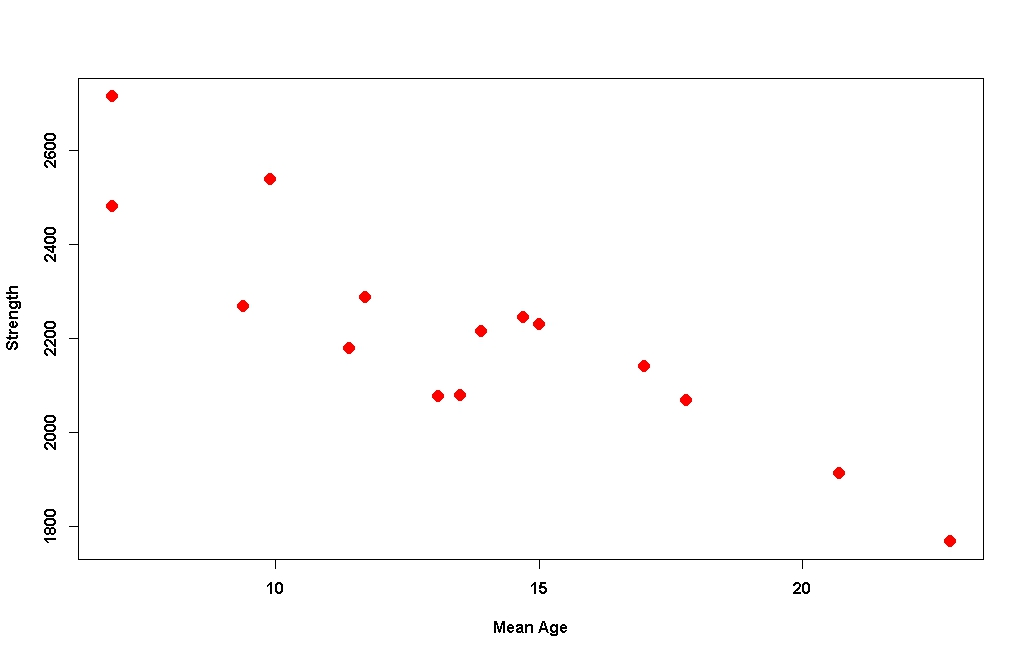
\includegraphics[scale=0.3]{images/12Aplot1}\\
\end{figure}


%----------------------------------------------------%

\subsection{Example 1 (c)}
\begin{itemize}
	\item What sort of relationship is indicated by this scatterplot?
	\item Strong or Weak?  - Quite Strong
	\item Positive or Negative?  - Negative
	\item Linear or Non-Linear - Seems to be linear
\end{itemize}

%----------------------------------------------------%

\subsection{Example 1 (d)}
Suppose we are given the following summations
\begin{itemize}
	\item $\sum X = 213.4$
	\item $\sum X^2 =3277.82$
	\item $\sum Y = 34122$
	\item $\sum Y^2 = 78547854$
	\item $\sum XY = 472203.9$
\end{itemize}
Compute the mean values of $X$ and $Y$.

\[ \bar{x} = \frac{\sum x}{n} = \frac{213.4}{15} = 14.226 \]

Similarly $\bar{y} =  2274.8$


%----------------------------------------------------%

\subsection{Example 1 (e)}
Compute the \textbf{Sum of Squares Identities} ($S_{XX}$ , $S_{YY}$ and $S_{XY}$).\\

\bigskip
From Formula Sheet (Back of Exam Paper)
\begin{eqnarray*}
	S_{XY} &=&
	\sum x_iy_i - \frac{\sum x_i\sum y_i}{n} = \left[472203.9 - \frac{213.4 \times 34122}{15} \right]=  -13238.42\\
	S_{XX} &=&
	\sum x_i^2 - \frac{(\sum x_i)^2}{n} = \left[3277.82 - \frac{213.4^2}{15}\right] =  241.8493\\
	S_{YY} &=&
	\sum y_i^2 - \frac{(\sum y_i)^2}{n} = \left[78547854 - \frac{34122^2}{15}\right] = 927128.4\\
\end{eqnarray*}



%----------------------------------------------------%

\subsection{Example 1 (f)}
Compute the \textbf{Correlation Coefficient} $r_{XY}$

\[r_{XY} =  \frac{S_{XY}}{\sqrt{S_{XX} \times S_{YY}}} \]

\[r_{XY} =  \frac{-13238.42}{\sqrt{241.8493 \times 927128.4}} \]
Remark : $\sqrt{XY} = \sqrt{X} \times \sqrt{Y}$.
\[r_{XY} =  \frac{-13238.42}{\sqrt{241.8493} \times \sqrt{927128.4}} \]
\[r_{XY} =  \frac{-13238.42}{15.55 \times 962.87} = \frac{-13238.42}{14972.63} = -0.8841 \]

This value is consistent with our interpretation of the scatterplot: Strong Negative Linear Relationship.

%----------------------------------------------------%


\subsection{Example 1 (g)}
Calculate the least squares regression line.\\
\bigskip
The least squares regression line comprises two important estimates:
\begin{itemize}
	\item  The slope estimate $b_1$
	\item  The intercept estimate $b_0$.
\end{itemize}
The least squares regression line has the following form:

\[ \hat{y}  = b_0 + b_1x \]

$\hat{y}$ is the \textbf{predicted} value for variables Y, when given a particular value $x$ for the predictor variable X.

%----------------------------------------------------%



\subsection{Example 1 (h)}

\begin{itemize}
	\item  The slope estimate $b_1$
	
	\begin{eqnarray*}
		b_1 = \frac{S_{XY}}{S_{XX}} = \frac{-13238.42}{241.8493} = -54.738
	\end{eqnarray*}
	
	\item  The intercept estimate $b_0$.
	\begin{eqnarray*}
		b_0 = \bar{y} -b_1\bar{x} = 2274.8 - (-54.738 \times 14.226) = 3053.503
	\end{eqnarray*}
\end{itemize}

\[ \hat{y}  = 3053.503 -54.738 x \]


%----------------------------------------------------%

\subsection{Example 1 (i)}
Interpret the values of the slope and the intercept.
\begin{itemize}
	\item  The slope estimate $b_1$ :  For each additional year in age, the shear strength of the bond decreases by approximately 54 units.
	\item The Intercept estimate $b_0$ : When the age of the propellant is 0 (i.e. brand new) the strength of the bond is expected to be 3053 units.
\end{itemize}
\bigskip
What is the estimate of the mean shear strength of the bond if the mean age of the propellants is 17 weeks?

\[ \hat{y}_{(x=17)}  = 3053.503 -54.738 \times 17 = 2122.96 \]

That looks plausible, from looking back at the scatter-plot.


%----------------------------------------------------%

\subsection{Example 1 (j)}

% image
% 12plot1
\begin{figure}
	% Requires \usepackage{graphicx}
	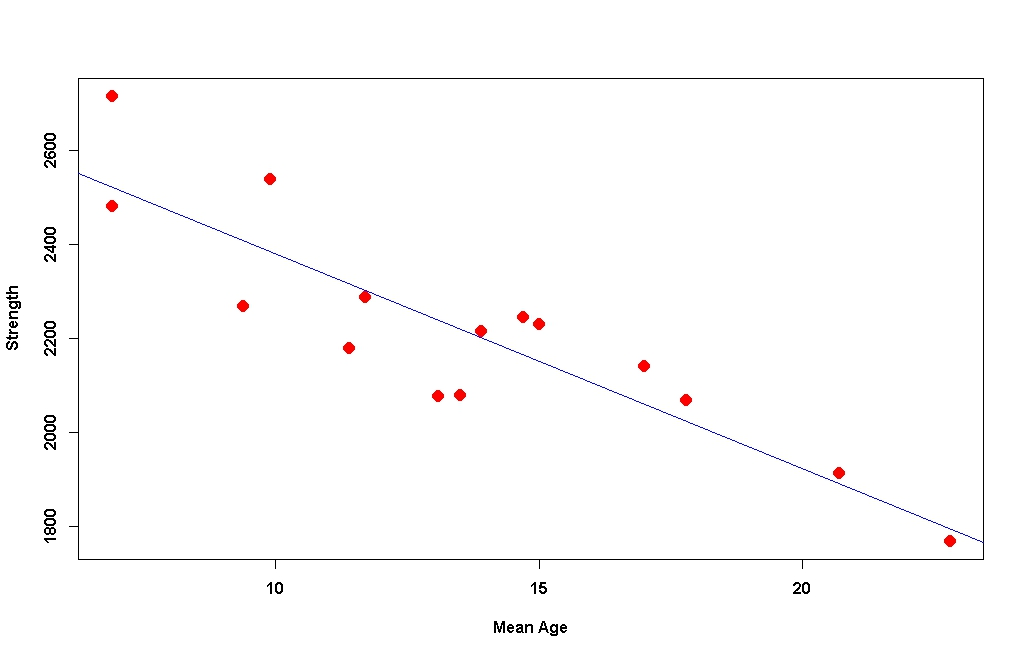
\includegraphics[scale=0.3]{images/12Aplot2}\\
\end{figure}


%----------------------------------------------------%

\subsection{Example 2 (a)}
(Spring 2010 Q5)\newline
A wood scientist wishes to determine if there is a relationship between the number of knots in a piece of wood and its tensile strength. A random selection of 8 timber beams were analysed and the results are given in the table (next slide).

%----------------------------------------------------%

\subsection{Example 2 (b)}
\begin{center}
	\begin{tabular}{|c|c|c|}
		\hline
		% after \\: \hline or \cline{col1-col2} \cline{col3-col4} ...
		Observation &Number of knots (x) &Tensile Strength \\
		&&N.MS (y)\\ \hline
		A &5&5\\
		B &8&2.9\\
		C &4&4.9\\
		D &9&2.8\\
		E &3&6.1\\
		F &6&4.1\\
		G &4&4.8\\
		H &7&3.2\\
		\hline
	\end{tabular}
\end{center}


%----------------------------------------------------%

\subsection{Example 2 (c)}
Computing summations: recommended approach is construction of a table.\\
\begin{center}
	\begin{tabular}{|c|c|c|c|c|c|}
		\hline
		Obs&$X$&$Y$&$X^2$&$Y^2$&$XY$\\
		A &5&5&&&25      \\
		B &8&2.9&&&23.2\\
		C &4&4.9&&&19.6\\
		D &9&2.8&&&25.2\\
		E &3&6.1&&&18.3\\
		F &6&4.1&&&24.6\\
		G &4&4.8&&&19.2\\
		H &7&3.2&&&22.4\\
		(sum)&46&33.8&&&177.5\\
		
		\hline
	\end{tabular}
\end{center}


%----------------------------------------------------%

\subsection{Example 2 (d)}

Summations from previous slide.
\begin{itemize}
	\item $\sum X = 46$
	\item $\sum X^2 =296$
	\item $\sum Y = 33.8$
	\item $\sum Y^2 = 152.56$
	\item $\sum XY = 117.5$
\end{itemize}
Compute the mean values of $X$ and $Y$.

\[ \bar{x} = \frac{\sum x}{n} = \frac{46}{8} = 5.75 \]

Similarly $\bar{y} =   4.225$


%----------------------------------------------------%

\subsection{Example 2 (f)}
Compute the \textbf{Sum of Squares Identities} ($S_{XX}$ , $S_{YY}$ and $S_{XY}$).\\
\bigskip
From Formula Sheet (Back of Exam Paper)
\begin{eqnarray*}
	S_{XY} &=&
	\sum x_iy_i - \frac{\sum x_i\sum y_i}{n} = -16.85\\
	S_{XX} &=&
	\sum x_i^2 - \frac{(\sum x_i)^2}{n} = 31.5\\
	S_{YY} &=&
	\sum y_i^2 - \frac{(\sum y_i)^2}{n} = 9.755\\
\end{eqnarray*}

%----------------------------------------------------%


\subsection{Example 2 (g)}
Compute the \textbf{Sum of Squares Identities} ($S_{XX}$ , $S_{YY}$ and $S_{XY}$).\\
\bigskip
From Formula Sheet (Back of Exam Paper)
\begin{eqnarray*}
	S_{XY} &=&
	\sum x_iy_i - \frac{\sum x_i\sum y_i}{n} = -16.85\\
	S_{XX} &=&
	\sum x_i^2 - \frac{(\sum x_i)^2}{n} = 31.5\\
	S_{YY} &=&
	\sum y_i^2 - \frac{(\sum y_i)^2}{n} = 9.755\\
\end{eqnarray*}



\subsection{Example 2 (h)}
Compute the regression estimates:
\begin{itemize}
	\item  The slope estimate $b_1$
	
	\begin{eqnarray*}
		b_1 = \frac{S_{XY}}{S_{XX}} = \frac{-16.85}{31.5} = -0.5349
	\end{eqnarray*}
	
	\item  The intercept estimate $b_0$.
	\begin{eqnarray*}
		b_0 = \bar{y} -b_1\bar{x} = 4.225 - (-0.5349 \times 5.75) = 7.300
	\end{eqnarray*}
\end{itemize}

\[ \hat{y}  = 7.300 -0.5349 x \]



%----------------------------------------------------%

\subsection{Example 2 (i)}

% image
% 12plot1
\begin{figure}
	% Requires \usepackage{graphicx}
	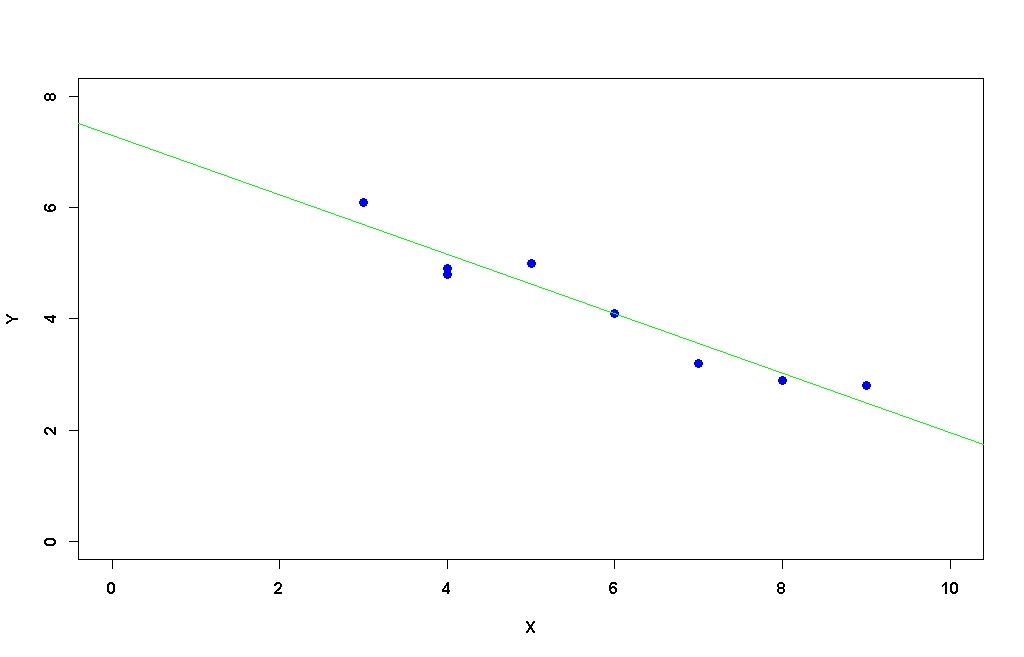
\includegraphics[scale=0.3]{images/12Aplot3}\\
\end{figure}


%-----------------------------------------------------------------%
\begin{verbatim}

X=rnorm(15,12.08,sd=4)

Y=rnorm(15,2200,sd=200)

while(cor(X,Y)>(-0.875))
{
	Y=rnorm(15,2200,sd=200)
}

X=round(X,1)
Y=floor(Y)


plot(X,Y,pch=17,col="blue",font.lab=2,font.axis=2,cex=1.6)
#
cor(X,Y)
sum(X)
sum(X^2)
sum(Y)
sum(Y^2)
sum(X*Y)


var(X)*(length(X)-1)
var(Y)*(length(Y)-1)
cov(X,Y)*(length(X)-1)
cor(X,Y)
coef(Y~X)
%-----------------------------------------------------------------
\end{verbatim}


\subsection{Density Curves}

Any curve that is always on or above the horizontal axis and has
total are underneath equal to one is a density curve.
\begin{itemize}
	\item Area under the curve in a range of values indicates the proportion of values in that range.
	\item Come in a variety of shapes, but the “normal” family of familiar
	bell-shaped densities is commonly used.
	\item Remember the density is only an approximation, but it simplifies analysis and is generally accurate enough for practical
	use.
\end{itemize}


\end{document}
